\documentclass[aspectratio=169]{beamer}
\usetheme{Bruno}
\usepackage{amsmath}
\usepackage{amssymb}
\usepackage{siunitx}
\usepackage{float}
\usepackage{tikz}
\def\checkmark{\tikz\fill[scale=0.4](0,.35) -- (.25,0) -- (1,.7) -- (.25,.15) -- cycle;} 
\usepackage{url}
\usepackage[siunitx,american,RPvoltages]{circuitikz}
\ctikzset{capacitors/scale=0.7}
\ctikzset{diodes/scale=0.7}
\usepackage{tabularx}
\newcolumntype{C}{>{\centering\arraybackslash}X}
\renewcommand\tabularxcolumn[1]{m{#1}}% for vertical centering text in X column
\usepackage{tabu}
\usepackage[spanish,es-tabla,activeacute]{babel}
\usepackage{babelbib}
\usepackage{booktabs}
\usepackage{pgfplots}
\usepackage{hyperref}
\hypersetup{colorlinks = true,
            linkcolor = black,
            urlcolor  = blue,
            citecolor = blue,
            anchorcolor = blue}
\usepgfplotslibrary{units, fillbetween} 
\pgfplotsset{compat=1.16}
\usepackage{bm}
\usetikzlibrary{arrows, arrows.meta, shapes, 3d, perspective, positioning,mindmap,trees,backgrounds}
\renewcommand{\sin}{\sen} %change from sin to sen
\usepackage{bohr}
\setbohr{distribution-method = quantum,insert-missing = true}
\usepackage{elements}
\usepackage{verbatim}
\usepackage[edges]{forest}
\usepackage{etoolbox}
\usepackage{schemata}
\usepackage{appendix}
\usepackage{listings}

\definecolor{color_mate}{RGB}{255,255,128}
\definecolor{color_plas}{RGB}{255,128,255}
\definecolor{color_text}{RGB}{128,255,255}
\definecolor{color_petr}{RGB}{255,192,192}
\definecolor{color_made}{RGB}{192,255,192}
\definecolor{color_meta}{RGB}{192,192,255}
\newcommand\diagram[2]{\schema{\schemabox{#1}}{\schemabox{#2}}}

\definecolor{codegreen}{rgb}{0,0.6,0}
\definecolor{codegray}{rgb}{0.5,0.5,0.5}
\definecolor{codepurple}{rgb}{0.58,0,0.82}
\definecolor{backcolour}{rgb}{0.95,0.95,0.92}

\lstdefinestyle{mystyle}{
    backgroundcolor=\color{backcolour},   
    commentstyle=\color{codegreen},
    keywordstyle=\color{magenta},
    numberstyle=\tiny\color{codegray},
    stringstyle=\color{codepurple},
    basicstyle=\ttfamily\footnotesize,
    breakatwhitespace=false,         
    breaklines=true,                 
    captionpos=b,                    
    keepspaces=true,                 
    numbers=left,                    
    numbersep=5pt,                  
    showspaces=false,                
    showstringspaces=false,
    showtabs=false,                  
    tabsize=2
}

\lstset{style=mystyle}
\title{Instrumentación I: \\ \emph{Introducción a la}\\ \emph{instrumentación industrial}}
\author{
    Juan J. Rojas, Hugo Sanchez Ortiz
}
\institute{Instituto Tecnológico de Costa Rica}
\date{\today}
\background{fig/background.jpg}
\begin{document}
\sisetup{unit-math-rm=\mathrm,math-rm=\mathrm} % change sinitx font
\sisetup{output-decimal-marker = {,}}
\maketitle

\newcommand{\blackandwhite}{black} %change this at the end

\begin{frame}{Señales}
    \begin{columns}[onlytextwidth]
        \begin{column}{0.6\textwidth}
        Cantidad física que varia con una o mas variables independientes y que porta información relevante.\\[8pt]
        Características: 
            \begin{itemize}
                \item Escalar o vectorial 
                \item Discreta o continua
                \item Determinista o aleatoria
            \end{itemize}    
        \end{column}
        \begin{column}{0.4\textwidth}
            \begin{center}
                \begin{tikzpicture}
                    \begin{axis}[
                        width= 0.9\linewidth,
                        height= 0.6\linewidth,
                        domain=0:4*pi,
                        samples=100,
                        ymin=-1.2, ymax=1.2,
                        xmin=0, xmax=4*pi+0.5,
                        axis x line=center,
                        axis y line=left,
                        ytick={\empty},
                        yticklabels={\empty},
                        xtick={\empty},
                        xticklabels={\empty},
                        %xtick={pi,2*pi,3*pi,4*pi},
                        %xticklabels={$\pi$,$2\pi$,$3\pi$,$4\pi$},
                        xlabel=$t$, % Set the labels
                        ylabel=$f(t)$,
                        x unit=, 
                        y unit=,
                        axis lines=center,
                        x label style={anchor=west},
                        y label style={anchor=south},
                        ]
                        \addplot[color=blue,mark=none,thick] {sin(deg(x))}
                    	;
                    \end{axis}
                    \begin{axis}[
                        yshift=-3cm,
                        width= 0.9\linewidth,
                        height= 0.6\linewidth,
                        domain=0:4*pi,
                        samples=100,
                        ymin=-1.2, ymax=1.2,
                        xmin=0, xmax=4*pi+0.5,
                        axis x line=center,
                        axis y line=left,
                        ytick={\empty},
                        yticklabels={\empty},
                        xtick={\empty},
                        xticklabels={\empty},
                        %xtick={pi,2*pi,3*pi,4*pi},
                        %xticklabels={$\pi$,$2\pi$,$3\pi$,$4\pi$},
                        xlabel=$p$, % Set the labels
                        ylabel=$f(p)$,
                        x unit=, 
                        y unit=,
                        axis lines=center,
                        x label style={anchor=west},
                        y label style={anchor=south},
                        ]
                        \addplot[color=blue,mark=none,thick] {rand}
                    	;
                    \end{axis}
                \draw[\blackandwhite] (-0.5,-3.2) rectangle (4,2.5);
                \end{tikzpicture}
            \end{center}
        \end{column}
    \end{columns}
\end{frame}

\begin{frame}{Estímulo}
Es la cantidad, propiedad o condición que se desea medir.\\[8pt]
Algunos ejemplos de estímulos: 
    \begin{itemize}
        \item Aceleración 
        \item Intensidad de radiación
        \item Temperatura
        \item Concentración de un componente químico
    \end{itemize}    
\end{frame}

\begin{frame}{Sistemas}
    \begin{columns}[onlytextwidth]
        \begin{column}{0.5\textwidth}
        Un sistema es una construcción o colección de diferentes elementos que juntos producen resultados que no pueden obtenerse con los elementos por separado\cite{INCOSE}.\\[8pt]
        Un sistema es un objeto o conjunto de objetos cuyas propiedades queremos estudiar\cite{modelica}.
        \end{column}
        \begin{column}{0.5\textwidth}
            \begin{center}
               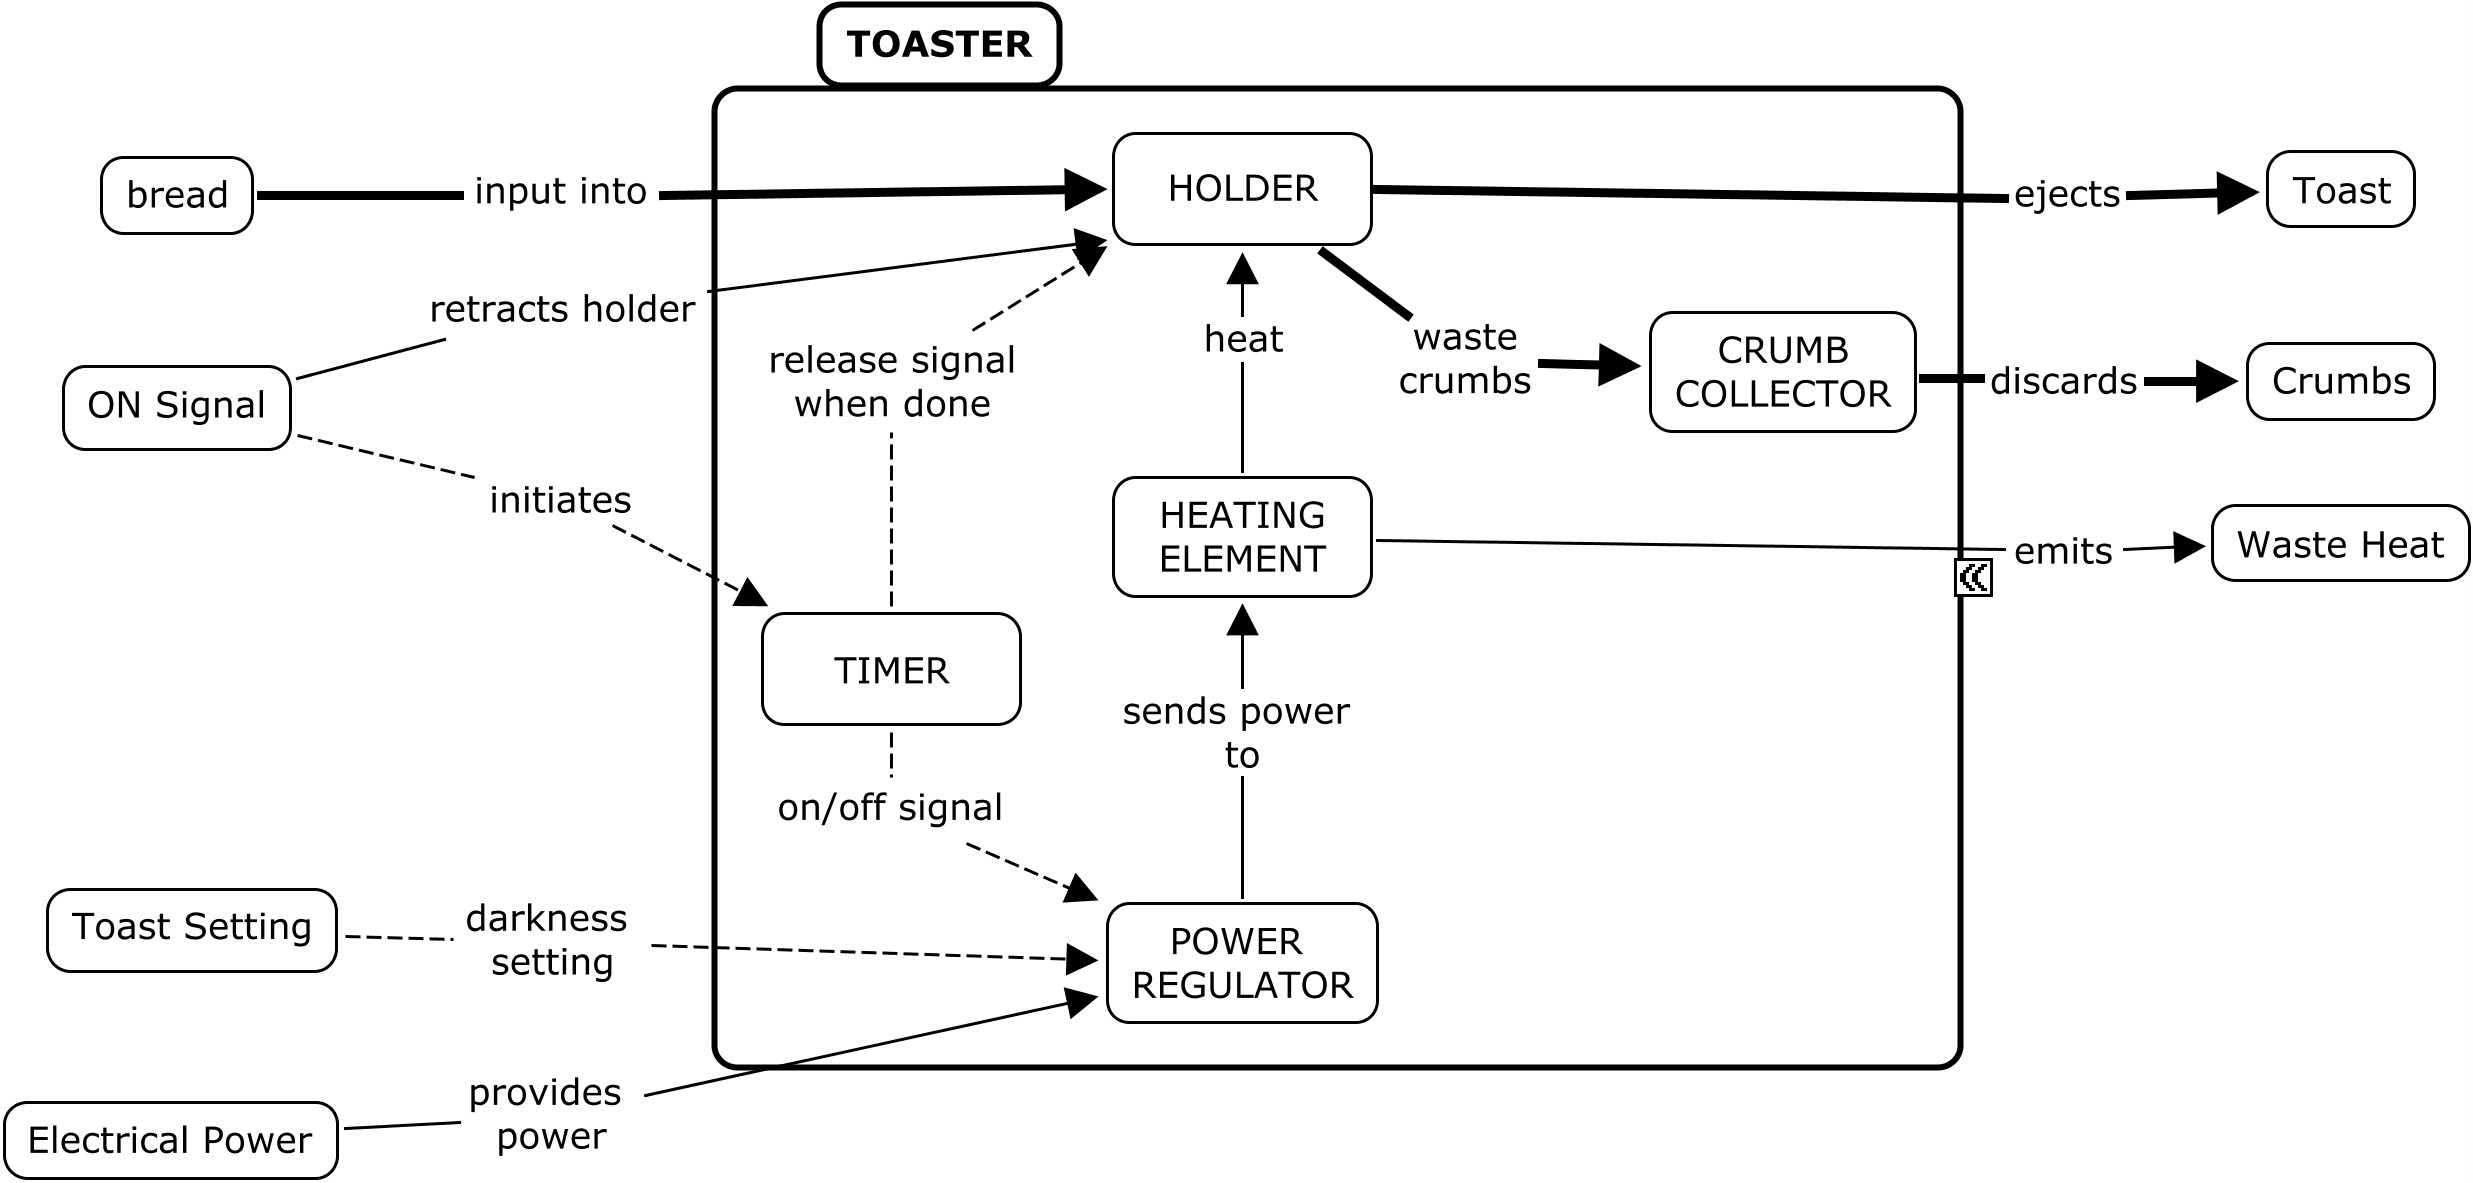
\includegraphics[width=\textwidth]{fig/tostadora.jpg}
               \scalebox{0.3}{\url{https://deseng.ryerson.ca/dokuwiki/_detail/design:toasterarchitecture.jpg?id=design\%3Asystem_diagram}}
            \end{center}
        \end{column}
    \end{columns}
\end{frame}

\begin{frame}{Señales de entrada y salida}
    \begin{columns}[onlytextwidth]
        \begin{column}{0.5\textwidth}
             \begin{itemize}
                \item Entradas: son las variables que afectan el comportamiento del sistema
                \item Salidas: son las variables que son definidas por el sistema
             \end{itemize}
        \end{column}
        \begin{column}{0.5\textwidth}
            \begin{center}
               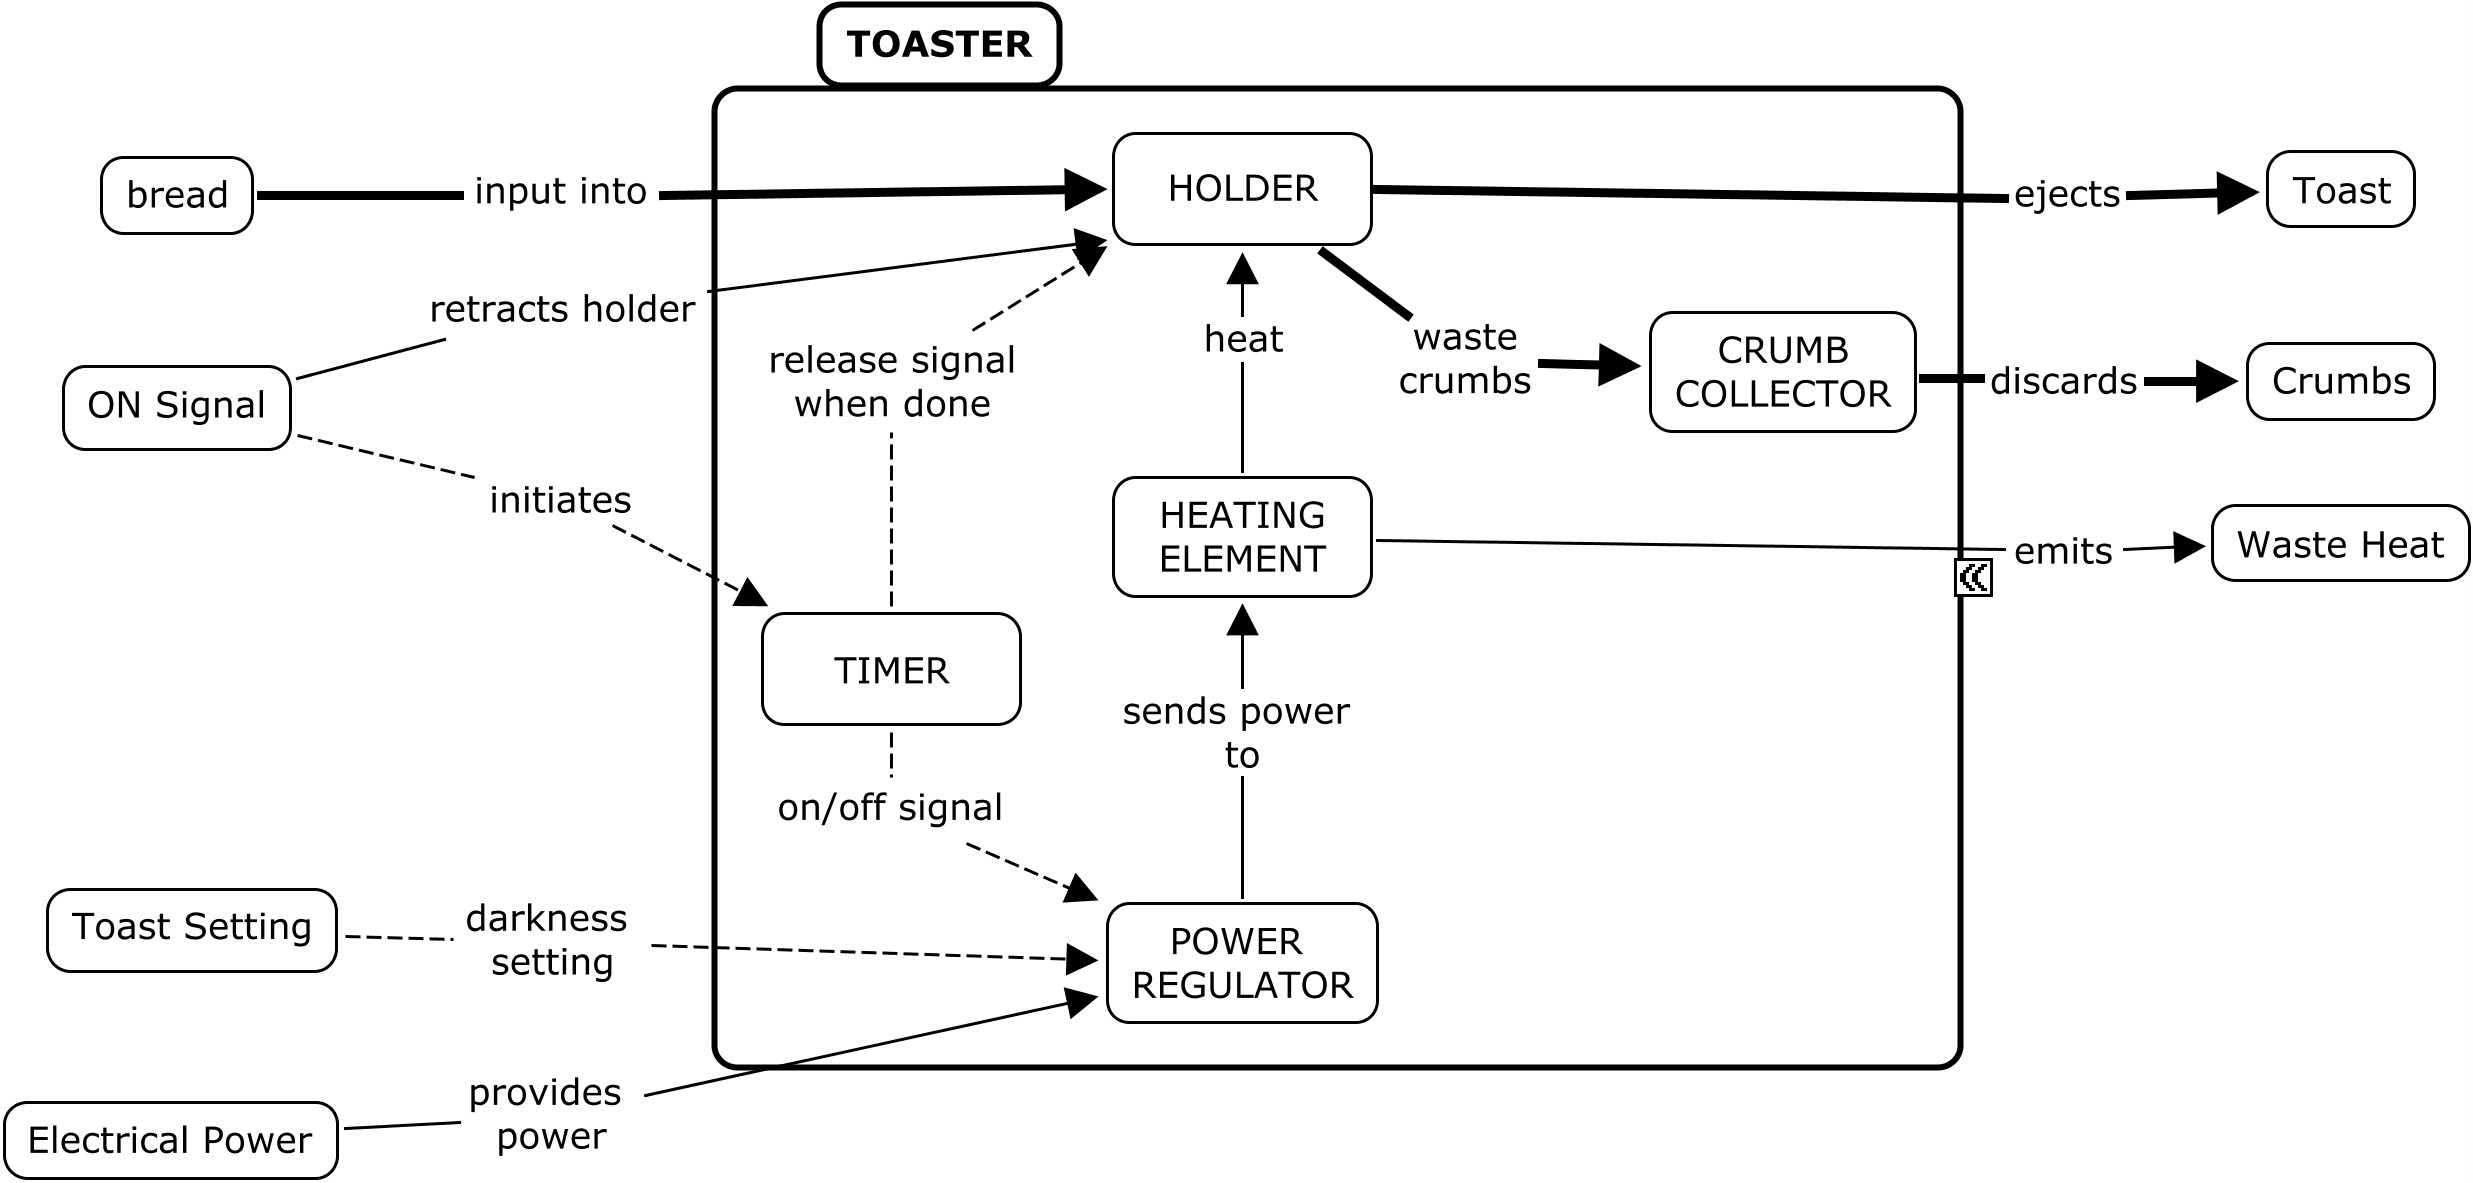
\includegraphics[width=\textwidth]{fig/tostadora.jpg}
               \scalebox{0.3}{\url{https://deseng.ryerson.ca/dokuwiki/_detail/design:toasterarchitecture.jpg?id=design\%3Asystem_diagram}}
            \end{center}
        \end{column}
    \end{columns}
\end{frame}

\begin{frame}{Modelos}
    \begin{columns}[onlytextwidth]
        \begin{column}{0.5\textwidth}
        Un modelo es una abstracción matemática de un sistema.\\[8pt]
        \begin{itemize}
            \item Se modela el sistema en base a ecuaciones
            \item Es una simplificación del sistema real
            \item Solo es valido en ciertas condiciones y/o rangos
        \end{itemize}
        
        
        \end{column}
        \begin{column}{0.5\textwidth}
            \begin{center}
               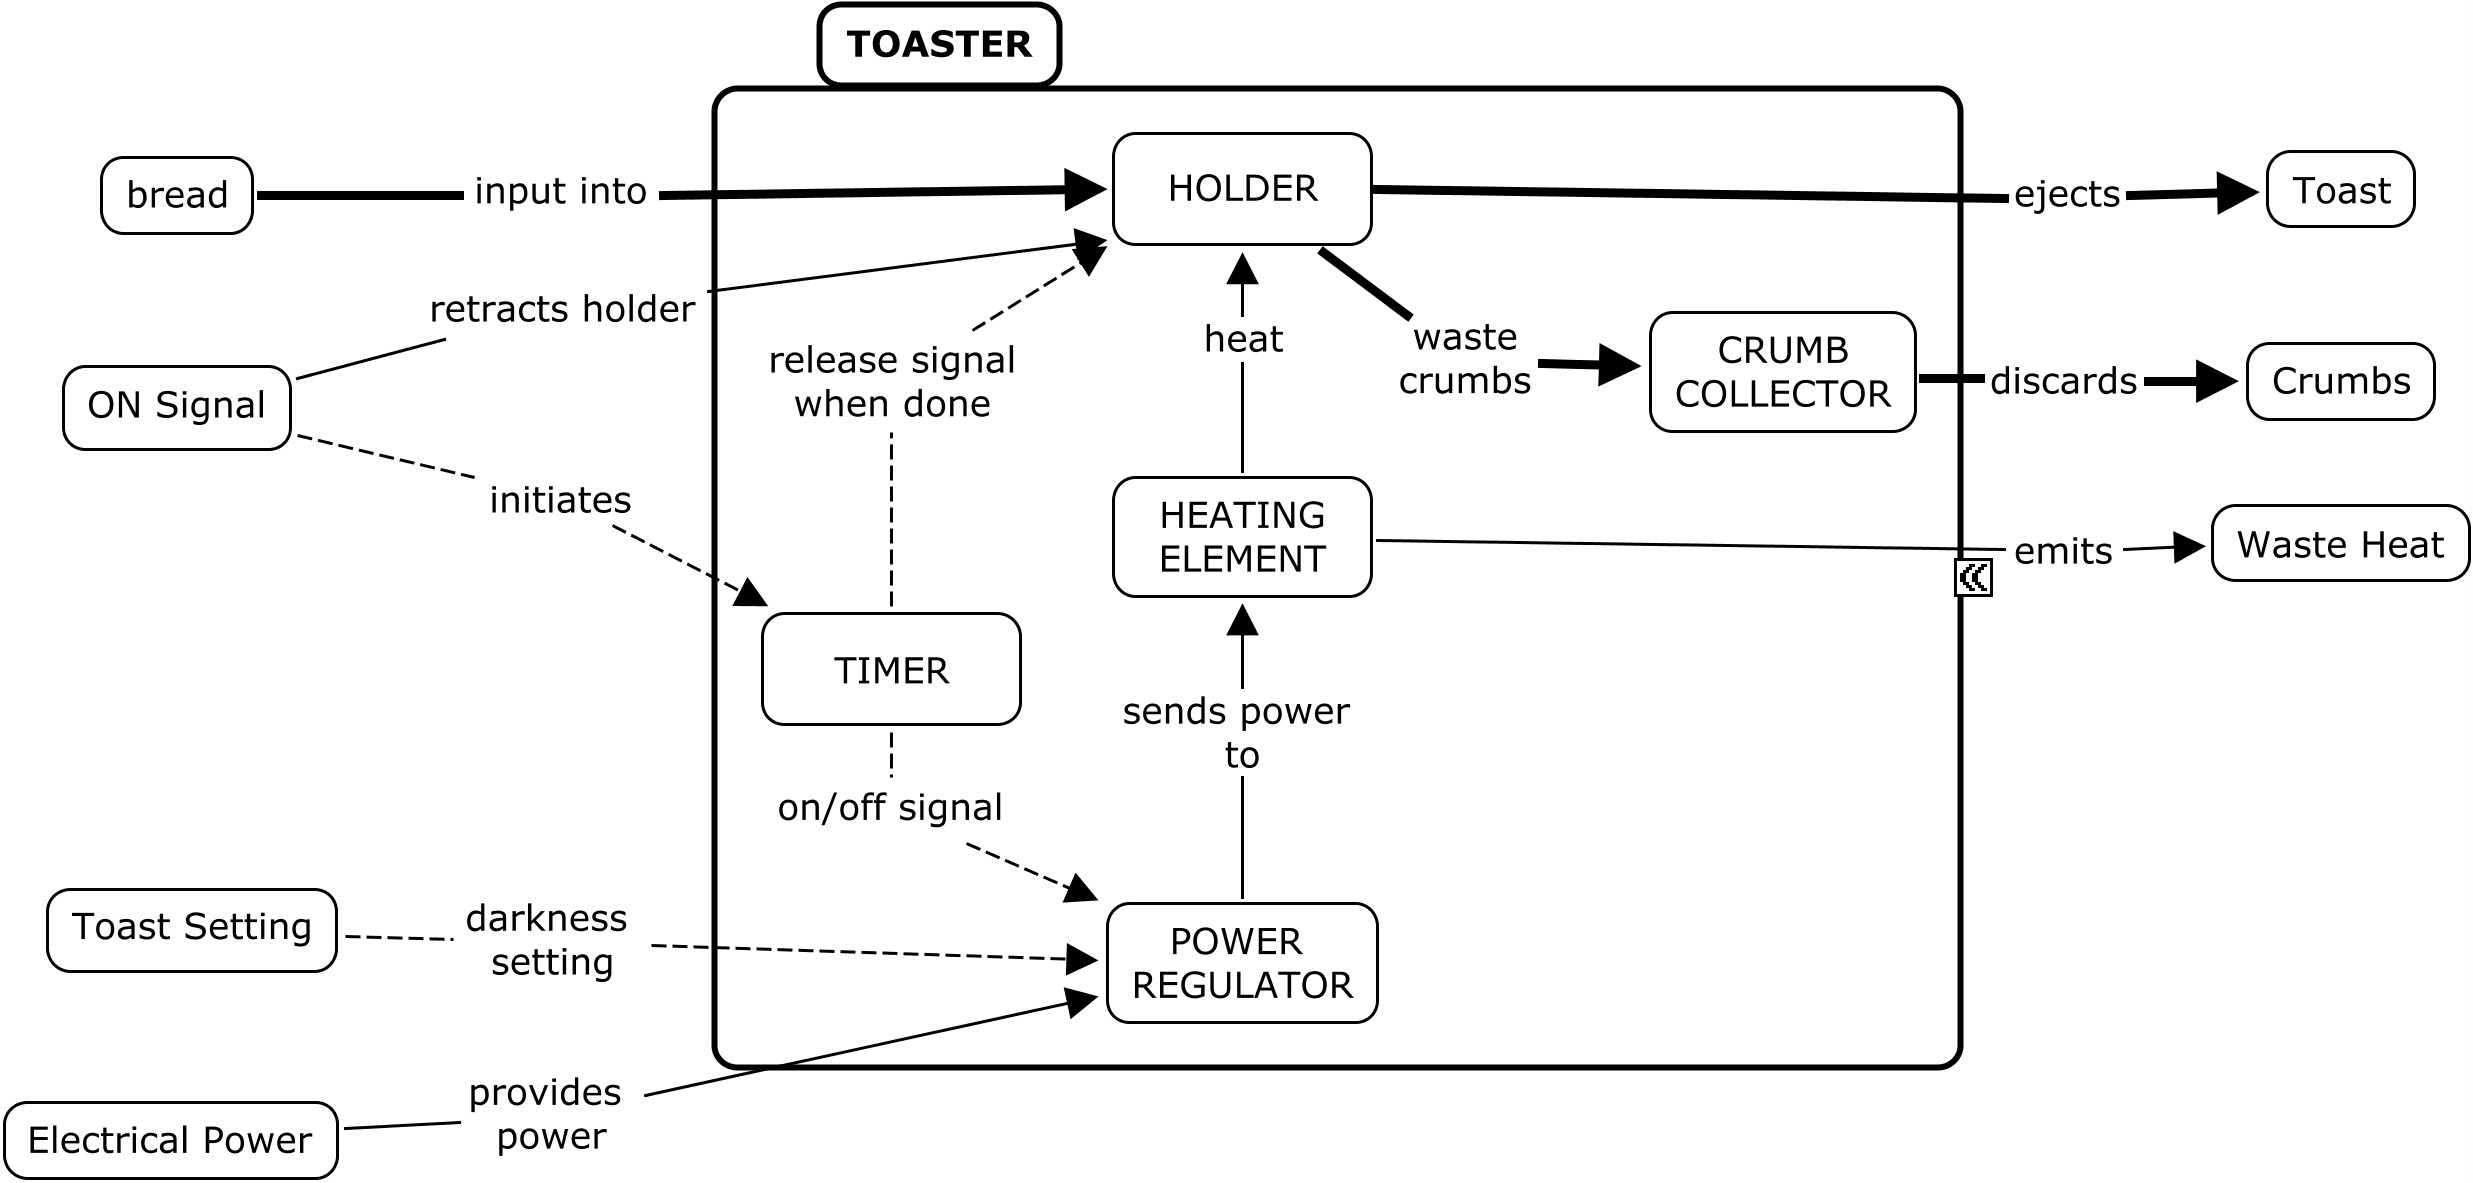
\includegraphics[width=\textwidth]{fig/tostadora.jpg}
               \scalebox{0.3}{\url{https://deseng.ryerson.ca/dokuwiki/_detail/design:toasterarchitecture.jpg?id=design\%3Asystem_diagram}}
            \end{center}
        \end{column}
    \end{columns}
\end{frame}


% \begin{frame}{Fuerza eléctrica} 
%     \begin{columns}[onlytextwidth]
%     \begin{column}{0.6\textwidth}
%         La fuerza eléctrica es la fuerza de atracción o repulsión entre dos cuerpos o partículas cargadas 
%         \begin{equation*}
%             F = k\dfrac{q_1q_2}{r^2}
%         \end{equation*}
%         donde $F$ es la fuerza eléctrica en newtons (\si{\newton}), $k$ es la constante de Coulomb ($\SI{9e9}{\newton \meter\squared / \coulomb \squared}$), $q_1$ y $q_2$ son dos cargas en coulombs (\si{\coulomb}), y $r$ es la distancia que separa a las cargas en metros (\si{\meter})   
%     \end{column}
%     \begin{column}{0.4\textwidth}
%         \begin{center}
%             \begin{tikzpicture}[scale=1]
%                 \shade[ball color=gray!10!] (0,0) coordinate(q1) circle (.4) node{$+q_1$};
%                 \shade[ball color=gray!10!] (2.5,0) coordinate(q2) circle (.4) node{$+q_2$};
%                 \draw[-latex,thick] (q1)++(-0.4,0)--+(-0.5,0);
%                 \draw[-latex,thick] (q2)++(0.4,0)--++(0.5,0);
%                 \draw[latex-,thick] (q1)++(0,1)--++(1,0);
%                 \draw[latex-,thick] (q2)++(0,1)--++(-1,0);
%                 \draw (q1)++(0,1)++(1.25,0)node{$r$};
%             \end{tikzpicture}\\[4pt]
%             \begin{tikzpicture}[scale=1]
%                 \shade[ball color=gray!10!] (0,0) coordinate(q1) circle (.4) node{$+q_1$};
%                 \shade[ball color=gray!10!] (2.5,0) coordinate(q2) circle (.4) node{$-q_2$};
%                 \draw[-latex,thick] (q1)++(0.4,0)--+(0.5,0);
%                 \draw[-latex,thick] (q2)++(-0.4,0)--++(-0.5,0);
%             \end{tikzpicture}\\[4pt]
%             \begin{tikzpicture}[scale=1]
%                 \shade[ball color=gray!10!] (0,0) coordinate(q1) circle (.4) node{$-q_1$};
%                 \shade[ball color=gray!10!] (2.5,0) coordinate(q2) circle (.4) node{$-q_2$};
%                 \draw[-latex,thick] (q1)++(-0.4,0)--+(-0.5,0);
%                 \draw[-latex,thick] (q2)++(0.4,0)--++(0.5,0);
%             \end{tikzpicture}
%         \end{center}
%     \end{column}
%     \end{columns}
% \end{frame}


\begin{frame}{Referencias}

\bibliographystyle{ieeetr}
\footnotesize
\bibliography{comunes/referencias}

\end{frame}

\end{document}